% ------------------------------------------------------------------------------
% TYPO3 Version 10 LTS - What's New (English Version)
%
% @author	Michael Schams <schams.net>
% @license	Creative Commons BY-NC-SA 3.0
% @link		https://typo3.org/help/documentation/whats-new/
% @language	English
% ------------------------------------------------------------------------------

\section{Introduction}
\begin{frame}[fragile]
	\frametitle{Introduction}

	\begin{center}\huge{\color{typo3darkgrey}\textbf{Introduction}}\end{center}
	\begin{center}\large{\textit{Key facts and figures about TYPO3 v10 LTS}}\end{center}

\end{frame}

% ------------------------------------------------------------------------------
% TYPO3 Version 10 LTS - The Facts

\begin{frame}[fragile]
	\frametitle{Introduction}
	\framesubtitle{TYPO3 Version 10 LTS}

	\begin{itemize}
		\item Release date: 21 April 2020
		\item Release type: LTS (long-term support)
	\end{itemize}

	\begin{figure}
		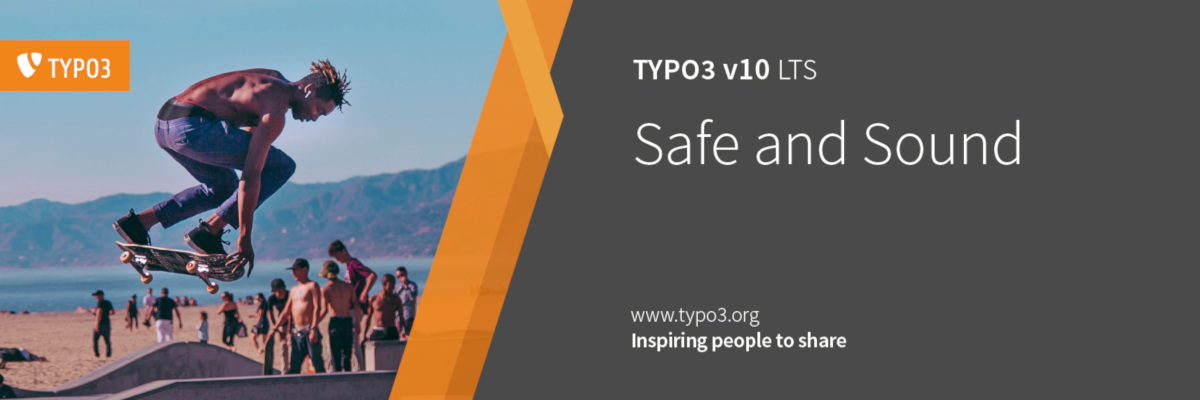
\includegraphics[width=0.95\linewidth]{Introduction/typo3-v10-4-banner.jpg}
	\end{figure}

\end{frame}

% ------------------------------------------------------------------------------
% TYPO3 Version 10 LTS - Executive Summary

\begin{frame}[fragile]
	\frametitle{Introduction}
	\framesubtitle{Executive Summary}

	\small
		TYPO3 v10.4 (also called TYPO3 v10 LTS indicating this is a long-term support version)
		is our new flagship and, without doubt, one of the most advanced PHP-based open-source
		content management systems on the market to date.

		\vspace{0.2cm}

		After publishing five sprint releases since July 2019, we can proudly claim that we
		have equipped TYPO3 with the top modern PHP libraries and that we have introduced some
		fantastic new enterprise features.

		\vspace{0.2cm}

		This document summarizes the most important changes between TYPO3 v9 LTS and v10 LTS
		from a technical perspective.

%		\vspace{0.2cm}
%
%		"What's New Slides" of all TYPO3 v10.x releases are available at
%		\href{https://typo3.org/help/documentation/whats-new/}{typo3.org}.

% changelog
% what's new slides

	\normalsize

\end{frame}

% ------------------------------------------------------------------------------
% System Requirements

\begin{frame}[fragile]
	\frametitle{Introduction}
	\framesubtitle{System Requirements}

	\begin{itemize}
		\item PHP version 7.2, 7.3 or 7.4
		\item PHP settings:

			\begin{itemize}
				\item \texttt{memory\_limit} >= 256M
				\item \texttt{max\_execution\_time} >= 240s
				\item \texttt{max\_input\_vars} >= 1500
				\item compilation option \texttt{-}\texttt{-disable-ipv6} must \underline{not} be used
			\end{itemize}

			\item Required PHP extensions:\newline
				\small
					filter, hash, openssl, pcre >= 8.38, session, SPL, standard,
					xml, zip and zlib
				\normalsize

		\end{itemize}

\end{frame}

% ------------------------------------------------------------------------------
% System Requirements

\begin{frame}[fragile]
	\frametitle{Introduction}
	\framesubtitle{System Requirements}

	\begin{itemize}
		\item Webserver such as Apache, Nginx, IIS, etc.
		\item All databases supported by \textbf{Doctrine DBAL} are also
			supported by TYPO3. For example:
	\end{itemize}

	\begin{figure}
		
\includegraphics[width=0.70\linewidth]{Introduction/logo-databases.png}
	\end{figure}

	\begin{itemize}
		\item Minimum disk space required: 200 MB
		\item The backend supports all modern browsers such as Microsoft Edge,
			Google Chrome, Firefox, Safari or any other compatible browser.
	\end{itemize}

\end{frame}

% ------------------------------------------------------------------------------
% Sprint Releases

\begin{frame}[fragile]
	\frametitle{Introduction}
	\framesubtitle{Development Timeline}

	Sprint Releases published:
	\vspace{0.4cm}
	\begin{itemize}
		\item v10.0 \tabto{1.1cm}23/Jul/2019\tabto{3.4cm}Pave the way for exciting new concepts and APIs
		\item v10.1 \tabto{1.1cm}01/Oct/2019\tabto{3.4cm}Routing Improvements and Site Handling v2
		\item v10.2 \tabto{1.1cm}03/Dec/2019\tabto{3.4cm}Fluid/Rendering Engine Improvements
		\item v10.3 \tabto{1.1cm}25/Feb/2020\tabto{3.4cm}Feature Freeze
		\item v10.4 \tabto{1.1cm}21/Apr/2020\tabto{3.4cm}LTS Release (long-term support)
	\end{itemize}

\end{frame}

% ------------------------------------------------------------------------------
% LTS Support Timeline

\begin{frame}[fragile]
	\frametitle{Introduction}
	\framesubtitle{Long-term Support}

	\begin{figure}
		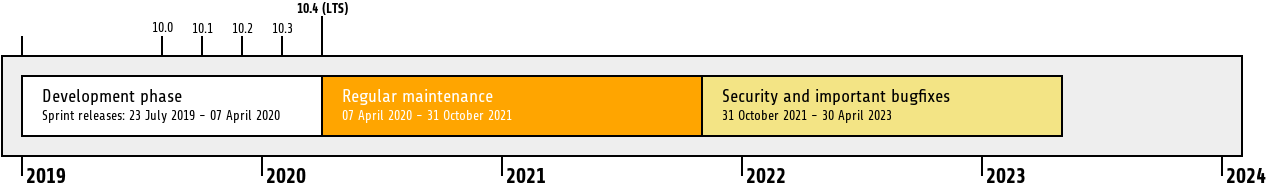
\includegraphics[width=1\linewidth]{Introduction/typo3-v10-lifecycle.png}
	\end{figure}

	\begin{itemize}
		\item TYPO3 version 10.4 is a LTS release (long-term support)
		\item Regular maintenance and bugfixes until October 2021
		\item Security and critical bugfixes until April 2023
	\end{itemize}
	\vspace{0.2cm}
	\textbf{Extended Support}\newline
	\smaller
		\href{https://typo3.com}{TYPO3 GmbH} offers extended long-term
			support (ELTS) for TYPO3 v10 LTS until April 2026.
	\normalsize

\end{frame}

% ------------------------------------------------------------------------------
